\section{Bildverarbeitung}\label{sec:linien}

Als haupts\"achliche Quelle f\"ur die Erfassung und Verarbeitung der Umwelt des Fahrzeugs wurde das Bild
einer Webcam verwendet. Eine Kinect-Kamera mit Tiefenbild war zwar bereits auf dem Fahrzeug vorinstalliert,
jedoch beschlossen wir aus folgenden Gr\"unden, eine eigene Kamera zu verwenden:
\begin{itemize}
	\item Der flache Blickwinkel der Kinect erlaubte es nicht, den Boden unmittelbar vor dem Fahrzeug
	zu sehen. Die von uns verwendete Webcam dagegen konnte frei angebracht und der Blickwinkel
	(insbesondere dessen Steilheit) nach Belieben variiert werden.
	\item Die OpenCV-Bibliothek bot uns die M\"oglichkeit, den Webcam-Stream direkt einzulesen und
	daran Voreinstellungen vorzunehmen. Bei der Kinect w\"are hingegen eine Vorkonvertierung n\"otig
	geworden.
	\item F\"ur die von uns zu realisierenden Aufgaben (Fahrbahn- und Schildererkennung) war die
	zus\"atzliche Tiefenbild-Funktionalit\"at der Kinect wenig bis nicht relevant.
\end{itemize}

\begin{figure}[h]
	\centering
	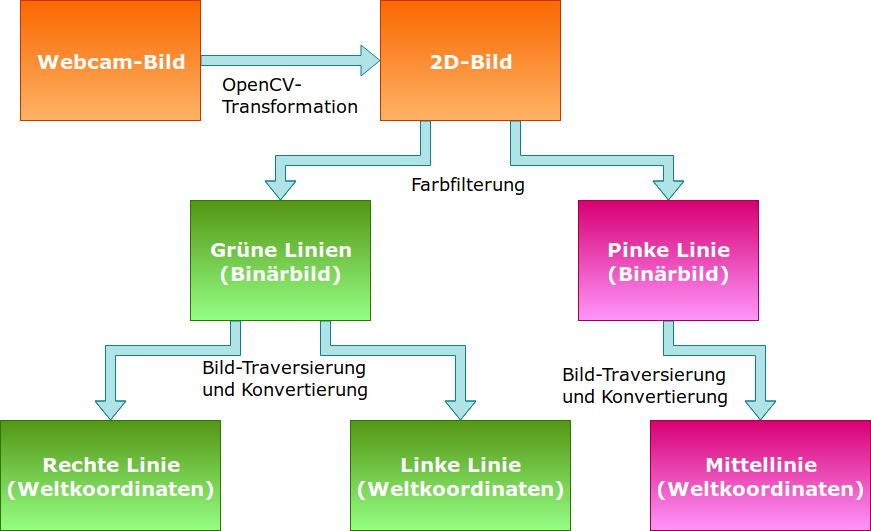
\includegraphics[width = 1.0\textwidth]{images/Bildverarbeitung.png}
	\caption{\"Ubersicht der einzelnen Schritte zur Bildverarbeitung}
	\label{fig:bildverarbeitung}
\end{figure}

Die groben Schritte, die im Rahmen der Bildverarbeitung durchgef\"uhrt werden, sind in
\figurename\ \ref{fig:bildverarbeitung} schematisch dargestellt.\\
Das eingelesene Webcam-Bild wird mithilfe der Bildverarbeitungs-Library OpenCV\cite{OCV} so transformiert, dass
der neue Bildausschnitt einer Draufsicht auf die Strecke aus der Vogelperspektive entspricht.
Davon ausgehend wird eine Farbfilterung vorgenommen, um die gr\"unen (Au\ss en-)Linien und die
pinke (innere) Linie jeweils in einem eigenen Bin\"arbild zu isolieren. Das Ergebnis wird
schlie\ss lich genutzt, um die Fahrzeugkoordinaten der einzelnen Linien zu bestimmen.\\
Die genauen Ma\ss nahmen, die f\"ur die Implementierung der einzelnen Verarbeitungsschritte getroffen 
wurden, werden im folgenden Abschnitt genauer vorgestellt.


\subsection{Kalibrierung der Kamera}

Beim Anbringen der Webcam wurde ein Blickwinkel gew\"ahlt, der zum einen eine m\"oglichst gute Sicht auf die
Strecke unmittelbar vor dem Fahrzeug erm\"oglicht, aber gleichzeitig ausreichend viel Strecke nach
vorne erfasst (auch um Verkehrsschilder noch gut erkennen zu k\"onnen).\\
Um eine korrekte Transformation des aufgenommenen Bildes (im Folgenden auch als \textit{3D-Bild} bezeichnet)
in die Vogelperspektive (nachfolgend auch als \textit{2D-Bild} bezeichnet) erzielen zu
k\"onnen, wurde eine Kalibrierung f\"ur die eingestellte Kamera-Position vorgenommen.

Zu diesem Zweck wurde zun\"achst ein Referenz-Rechteck aus Papier angefertigt und dessen Ma\ss e
in Zentimetern ausgemessen.
F\"ur die Kalibrierung wurde dieses im zentralen Sichtfeld der Kamera platziert, zus\"atzlich wurde der
Abstand zum Fahrzeug bestimmt (siehe \figurename\ \ref{fig:testrechteck}).

\begin{figure}[h]
	\centering
	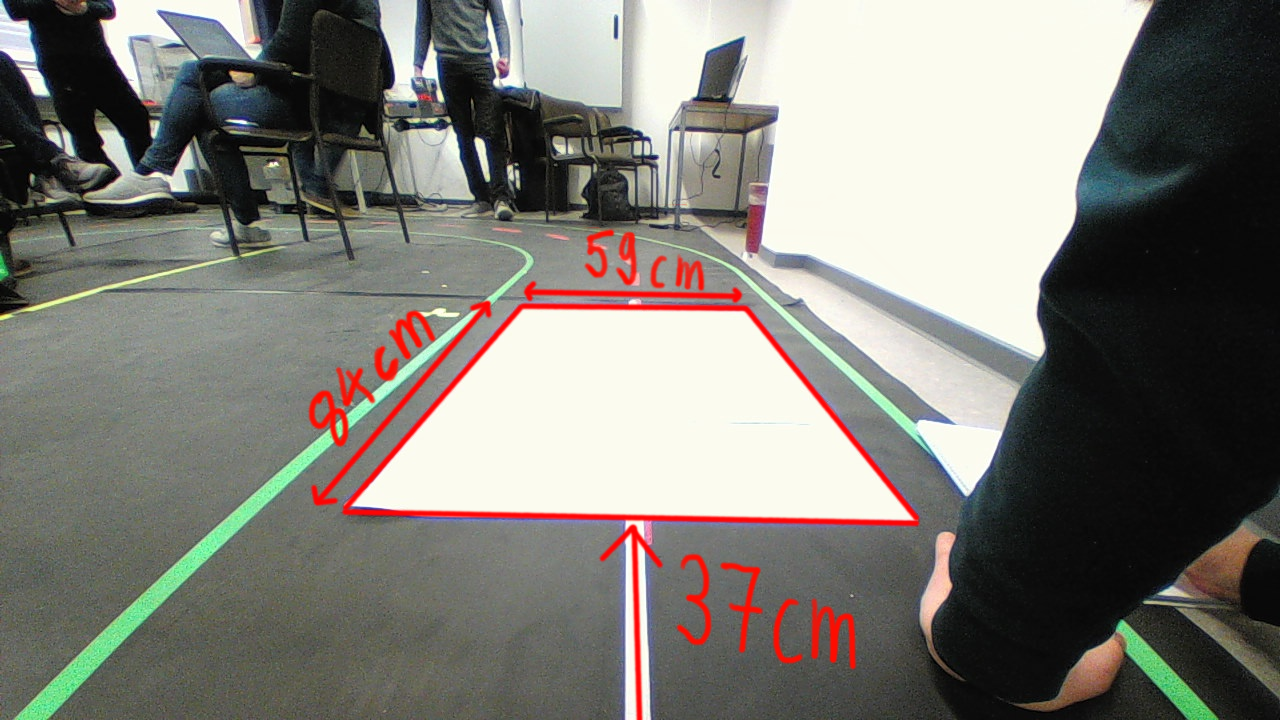
\includegraphics[width = 0.7\textwidth]{images/Testrechteck.png}
	\caption{Kalibrierung der Kamera mit dem Referenz-Rechteck}
	\label{fig:testrechteck}
\end{figure}

Anschlie\ss end wurden im aufgenommenen Bild die Pixelkoordinaten der Eckpunkte des Rechtecks ermittelt und notiert.

Zur Repr\"asentation einer festen Kamera-Kalibrierung und damit verkn\"upfter Informationen wurde eine eigene
C++-Klasse \texttt{CameraCalibration} geschrieben. Auf diese Weise l\"asst sich eine Kalibrierung leicht an mehreren
Stellen im Code verwenden. Instanzen der Klasse werden bei der Initialisierung einmalig
mit den ausgemessenen Pixelkoordinaten, den realen Ma\ss en des verwendeten Referenz-Rechtecks, dem gew\"unschten
Verh\"altnis von Pixeln zu Zentimetern im 2D-Bild sowie dem darzustellenden
Ausschnitt der Realit\"at in Zentimetern (in Blickrichtung und zu den beiden Seiten links
und rechts) initialisiert.\\
Davon ausgehend werden automatisch alle weiteren zur Erzeugung des Zielbildes n\"otigen Parameter berechnet.
Insbesondere wird \"uber die OpenCV-Funktion \texttt{getPerspectiveTransform} eine Transformationsmatrix
und deren Inverse abgespeichert, die jedem Pixel in der 3D-Perspektive eine Koordinate im 2D-Bild zuordnet
und umgekehrt.

\subsubsection{Umrechnung von Koordinaten}

Durch Anwendung der ermittelten Transformationsmatrix lassen sich einzelne Punkte des Webcam-Bilds zwar
in die Vogelperspektive mappen, jedoch war f\"ur die sp\"atere einfache Weiterverarbeitung von ermittelten Punkten
der Fahrbahnmarkierungen in der Fahrzeugregelung gew\"unscht, dass diese in Fahrzeugkoordinaten vorliegen.
Zu diesem Zweck musste eine Anpassung des Koordinatensytems sowie der verwendeten Einheiten vorgenommen
werden. Der Unterschied zwischen 2D-Bild-Koordinaten und den entsprechenden Koordinaten der realen
Welt ist in \figurename\ \ref{fig:koordinatensysteme} grafisch dargestellt.

\begin{figure}[h]
	\centering
	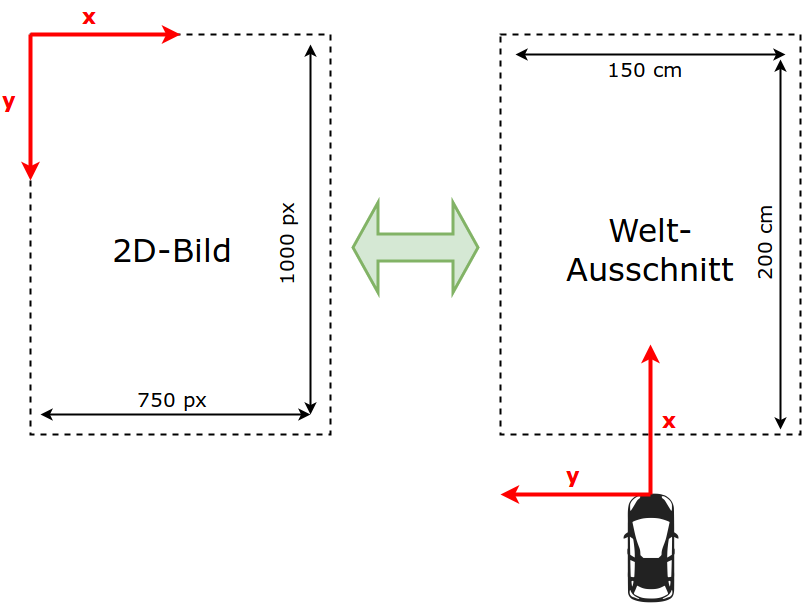
\includegraphics[width = 0.8\textwidth]{images/Koordinatenumrechnung.png}
	\caption{2D-Bild- vs. Fahrzeugkoordinaten}
	\label{fig:koordinatensysteme}
\end{figure}

Die ben\"otigte Funktionalit\"at zur Umrechnung zwischen 2D-Bild- und Welt-Koordinaten wird durch
Methoden in der Klasse \texttt{CameraCalibration} zur Verf\"ugung gestellt. Dabei werden die bei der Kalibrierung
abgespeicherten Informationen \"uber Gr\"o\ss e und Positionierung des Referenz-Rechtecks sowie der
Skalierungsfaktor f\"ur Pixel / Zentimeter verwendet
und das Koordinatensystem passend dazu neu bestimmt und ausgerichtet.\\

\textbf{TODO}\\
- Umrechnung der Koordinatensysteme ineinander, Formeln?\\

\subsection{Einlesen des Kamera-Bilds}

Zum Einlesen von Bildern der Webcam wurde ein Objekt vom OpenCV-Typ \texttt{VideoCapture} verwendet.
Dieses wurde in einer eigenen Klasse \texttt{CameraReader} gekapselt und um Zusatzfunktionalit\"at
erg\"anzt. So stellte sich heraus, dass zu jedem Auslesezeitpunkt f\"unf Webcam-Frames im Buffer des
Video-Streams gehalten werden, wovon das aktuellste das \"alteste ist. Um das neueste zu verwenden
und Lags zu vermeiden, verwirft der \texttt{CameraReader} daher die ersten vier Frames, sodass nur das letzte
tats\"achlich ausgelesen und im OpenCV-Bildformat (als \texttt{Mat}-Objekt) zur\"uckgegeben wird.

Zus\"atzlich wurde eine Methode zur Einstellung der Helligkeit, des Kontrasts, der S\"attigung und des
Farbtons des Kamera-Streams implementiert, um die Aufnahme bestm\"oglich auf aktuelle Lichtverh\"altnisse und zu
detektierende Farben anpassen zu k\"onnen.

Um eine modulare Softwarearchitektur zu gew\"ahrleisten, wurde die Funktionalit\"at zum Auslesen der Webcam
in eine eigene ROS-Node \texttt{webcam\_publisher} ausgelagert, welche den
\texttt{CameraReader} verwendet und ausgelesene Frames als ROS-Messages \"uber das ROS-Topic
\texttt{camera/frame} published.

\subsection{Weiterverarbeitung des Kamera-Bilds}

Das Herzst\"uck der eigentlichen Bildverarbeitung bildet die Klasse \texttt{ImageProcessor}. Sie kapselt
ein OpenCV-\texttt{Mat}-Objekt und enth\"alt verschiedene, zu gro\ss em Teil auf OpenCV basierende
Operationen, die darauf (in teilweise beliebiger
Reihenfolge) ausgef\"uhrt werden k\"nnen. Insbesondere stellt sie die Funktionalit\"at bereit, um

\begin{itemize}
	\item eine Transformation des Bildes in die Vogelperspektive anhand eines gegebenen
	\texttt{CameraCalibration}-Objekts vorzunehmen. Die Dimensionen des erzeugten Bilds bestimmen sich aus
	den in der Kalibrierung enthaltenen Informationen.
	\item eine Konvertierung des Bildes in den HSV-Farbraum vorzunehmen. Das aufgenommene Bild liegt
	zun\"achst in RGB vor, f\"ur die Bestimmung und Eingrenzung von Farb-Schwellwerten zur Linienerkennung
	ist HSV jedoch geeigneter: W\"ahrend (S)aturation und (V)alue angeben,
	wie \glqq wei\ss \grqq\ oder \glqq schwarz\grqq\ ein Pixel
	sein soll, l\"asst sich der Farbton durch den (H)ue-Kanal genau einstellen und auf einen engen
	Durchlassbereich begrenzen, was mit RGB nicht so leicht m\"oglich w\"are.
	\item eine Farbfilterung (nach einer vorherigen Transformation in den HSV-Farbraum) vorzunehmen. Dazu
	werden zwei Schwellwerte f\"ur die einzelnen Farbkan\"ale angegeben, die jeweils die untere bzw. die
	obere Schranke f\"ur den H-/S-/V-Wert darstellen. Das Ergebnis der Filterung ist ein Graustufen-Bild,
	in dem nur diejenigen Pixel wei\ss\ sind, deren Werte f\"ur \textit{alle} Kan\"ale zwischen den
	jeweiligen Schwellwerten liegen. Alle anderen Pixel sind dagegen schwarz (bzw. haben den Wert 0).
	Werden die Schwellwerte korrekt gew\"ahlt, lassen sich auf diese Weise gerade die rechte und linke
	Au\ss enlinie bzw. die Mittellinie der Fahrbahn in je einem Bin\"arbild isolieren.
	\item wei\ss e / nicht schwarze Punkte in einem (Bin\"ar-)Bild in einer bestimmten Pixel-Reihe
	von einer vorgegebenen Seite des Bildes aus zu suchen und die Pixel-Koordinaten zur\"uckzugeben.
	Diese Funktionalit\"at wird sp\"ater zur Ermittlung von Linienpunkten ben\"otigt.
\end{itemize} 

\textbf{TODO}\\
- nebeneinander dargestellt und kurz beschrieben: Quellbild - 2D-Bild - 2D-Bin\"arbild\\

\subsection{Detektion der Fahrbahnlinien}

F\"ur die Detektion der Fahrbahnlinien wurde eine abstrakte Oberklasse \texttt{LaneDetector} implementiert,
welche Methoden zur Ermittlung bzw. R\"uckgabe der einzelnen Linien deklariert und daf\"ur Objekte
weiterer Klassen verwendet. Die Idee hinter dieser
abstrakten Klasse war es, durch unterschiedliche Implementierungen Linienpunkte auf verschiedene Weise,
aber \"uber das gleiche Interface ermitteln zu k\"onnen.\\

\begin{figure}[h]
	\centering
	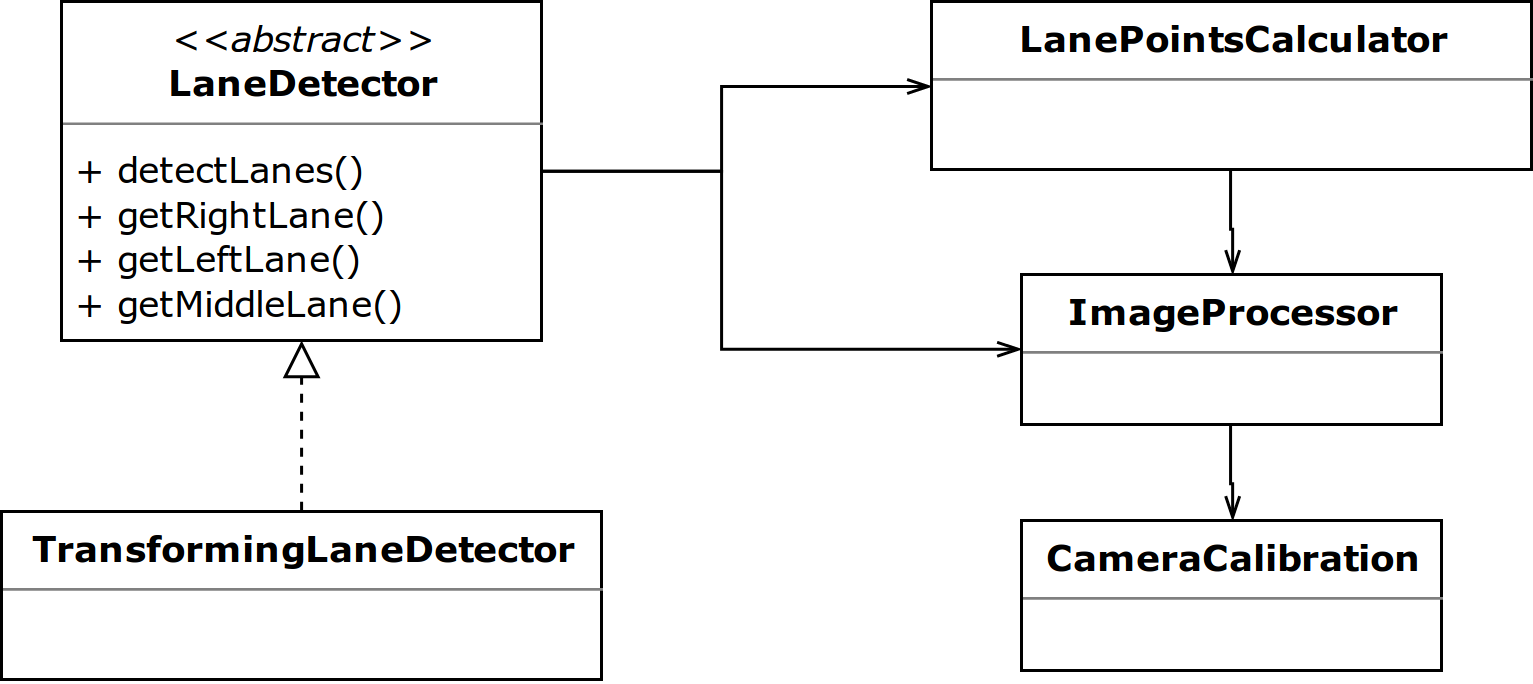
\includegraphics[width = 1.0\textwidth]{images/LaneDetectionKlassendiagramm.png}
	\caption{Vereinfachtes Klassendiagramm der Klassen zur Liniendetektion}
	\label{fig:lanedetection}
\end{figure}

Die f\"ur die Liniendetektion relevanten Klassen sind in \figurename\ \ref{fig:lanedetection} vereinfacht
dargestellt.

Die Singleton-Klasse \texttt{LanePointsCalculator} enth\"alt verschiedene Methoden, um mithilfe eines
\"ubergebenen \texttt{ImageProcessor}-Objekts Linien-Punkte im Bin\"arbild zu ermitteln. Bei der
Verwendung ist darauf zu achten, dass der \texttt{ImageProcessor} bereits ein fertig verarbeitetes
Graustufen-Bild enth\"alt.

Konkret implementiert wurden die Methoden aus \texttt{LaneDetector} in der Klasse
\texttt{TransformingLaneDetector}.\\
Diese verwendet zun\"achst den \texttt{ImageProcessor}, um das Quellbild in 2D zu transformieren und zwei
farbgefilterte Bilder (eines mit den gr\"unen und eines mit den pinken Linien) zu erhalten. Im n\"achsten
Schritt werden die Pixelkoordinaten der Linien mithilfe der Instanz des \texttt{LanePointsCalculator}
ermittelt und zwischengespeichert. Die endg\"ultigen Punkte der Linien in Pixelkoordinaten ergeben sich
erst aus einer Filterung der Zwischenergebnisse. Hier werden die Abst\"ande der gr\"unen Linien-Punkte
von der Mittellinie betrachtet, um sicherzustellen, dass es sich tats\"achlich um einen linken bzw.
rechten Punkt handelt (und nicht durch ein zwischenzeitlich schlechtes Bild Punkte der jeweils
gegen\"uberliegenden Linie falsch zugeordnet wurden). Nur Punkte, die rechts bzw. links von der
Mittellinie liegen, werden auch tats\"achlich als der entsprechenden Au\ss enlinie zugeh\"orig erkannt.

Schlie\ss lich wird das gespeicherte \texttt{CameraCalibration}-Objekt verwendet, um aus den Pixelkoordinaten
der jeweiligen Linie die entsprechenden Fahrzeugkoordinaten zu berechnen und zur\"uckzugeben.\\

F\"ur den Betrieb der Linienerkennung im Gesamtsystem existiert die ROS-Node \texttt{lane\_detection},
welche das ROS-Topic \texttt{camera/frame} subscribed und so die einzelnen Frames, die vom
\texttt{webcam\_publisher} ver\"offentlicht werden, empf\"angt. Zus\"atzlich werden die Farbschwellwerte
\"uber \texttt{rqt\_reconfigure}\ref{TODO: Link zu rqt_reconfigure} empfangen und gesetzt und zusammen mit
dem aktuellsten Frame an eine Instanz des \texttt{TransformingLaneDetector} \"ubergeben, welcher die
eigentlichen Berechnungen vornimmt.

Die ermittelten Punkte der einzelnen Fahrbahnlinien in Fahrzeugkoordinaten werden dann \"uber die Topics
\texttt{right\_lane}, \texttt{left\_lane} und \texttt{middle\_lane} gepublished, um von der
Trajektorienberechnung weiterverwendet werden zu k\"onnen. Au\ss erdem wird ein Bin\"arbild des fertig
verarbeiteten Webcam-Frames zu Monitoring-Zwecken ebenfalls gepublished.